\documentclass[12pt,a4paper]{article}
\usepackage[utf8]{inputenc}
\usepackage[norsk]{babel}
\usepackage{amsmath, amssymb, amsthm}  % For matematisk notasjon
\usepackage{algorithm, algorithmic}    % For å skrive algoritmer
\usepackage{graphicx}                  % For å inkludere bilder
\usepackage{hyperref}                  % For hyperlenker
\usepackage{pgfplots}                  % For grafer
\usepackage{float}
\pgfplotsset{compat=1.16}

\title{Øving 5 - Algoritmer og Datastrukturer}
\author{Henrik Halvorsen Kvamme}
\date{\today}

\begin{document}

\maketitle

\section{Introduksjon}
Denne øvingen har 2 deloppgaver som må gjøres. Den første ber deg lese fra en fil med navn til alle som tar algdat faget for å legge inn navnene som nøkler til et hashmap med lenka lister.

Deloppgave 2 ber deg lage to implementasjoner av hashmap med unike tall som nøkler. Implementasjonene bruker to former for addressering: lineær probering og dobbel hashing. For et den skal godkjennes må m være minst 10 000 000. Man må også teste ulike fyllingsgrader. De må også telle antall kollisjoner. Til slutt skal du trekke konklusjon fra funnene.

\section{Teori}
For at hashmap implementasjonene skal være effektive bør de ha en god hashfunksjon. En hashfunksjon tar inn en verdi og omformer den til å bli en tallverdi slik at den kan brukes som index til en tabell.

For deloppgave to gjør jeg dette ved å multiplisere verdien med et primtal og tar så modulus av størrelsen til tabellen. Tabellstørrelsen bør helst være et primtal. Jeg satt det til å være det nærmeste primtallet over 10 000 000 for å møte kravet, altså m = 10 000 019.

\newpage

\section{Resultater}
Etter omntrent ett minutt ender LinearProbing på omntrent index = 9989405 av m = 10000019.
Dette er fordi hashfunksjonen er dårlig, og det er for mange kollisjoner. Vi måler derfor ikke tiden når den er 100% fylt.

\begin{table}[H]
    \centering
    \caption{Her ser du målingene for hashmap implementasjonene per fyllingsgrad.}
    \label{table:performance}
    \begin{tabular}{|c|c|c|c|}
    \hline
    Method & \% of \( m \) inserted & Time (ms) & Collisions \\
    \hline
    \hline
    Linear Probing & 50 & 227 & 2,450,043 \\
    Linear Probing & 80 & 542 & 15,601,418 \\
    Linear Probing & 90 & 723 & 38,560,263 \\
    Linear Probing & 99 & 1796 & 293,414,184 \\
    \hline
    Double Hashing & 50 & 278 & 1,925,374 \\
    Double Hashing & 80 & 611 & 8,286,508 \\
    Double Hashing & 90 & 778 & 14,800,364 \\
    Double Hashing & 99 & 1109 & 46,712,940 \\
    Double Hashing & 100 & 27613 & 788,629,257 \\
    \hline
    \end{tabular}
\end{table}

\begin{figure}[H]
    \centering
    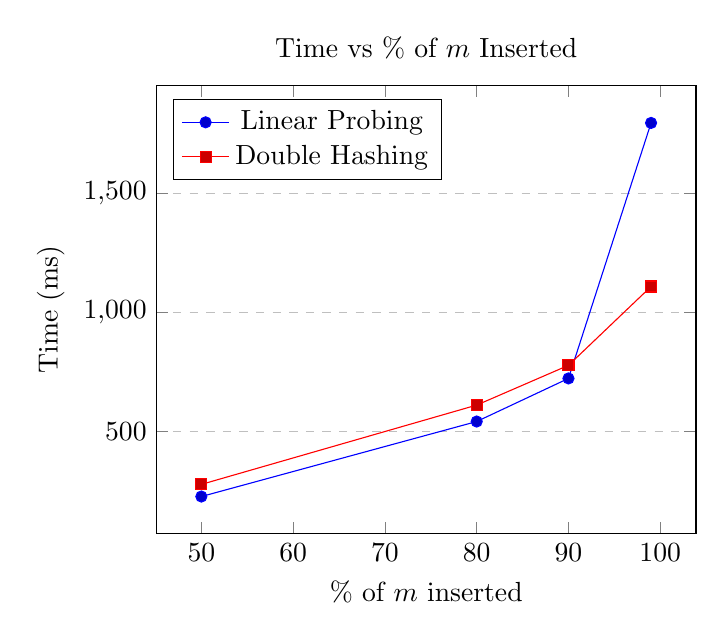
\begin{tikzpicture}
        \begin{axis}[
            title={Time vs \% of \( m \) Inserted},
            xlabel={\% of \( m \) inserted},
            ylabel={Time (ms)},
            legend pos=north west,
            ymajorgrids=true,
            grid style=dashed,
        ]
        
        \addplot coordinates {
            (50, 227)
            (80, 542)
            (90, 723)
            (99, 1796)
        };
        \addlegendentry{Linear Probing}
        
        \addplot coordinates {
            (50, 278)
            (80, 611)
            (90, 778)
            (99, 1109)
        };
        \addlegendentry{Double Hashing}
        
        \end{axis}
    \end{tikzpicture}
    \caption{Forholdet mellom tid og fyllingsgrad ser ut til å begynne lineært, men blir eksponentiell.}
    \end{figure}
    
    \begin{figure}[H]
    \centering
    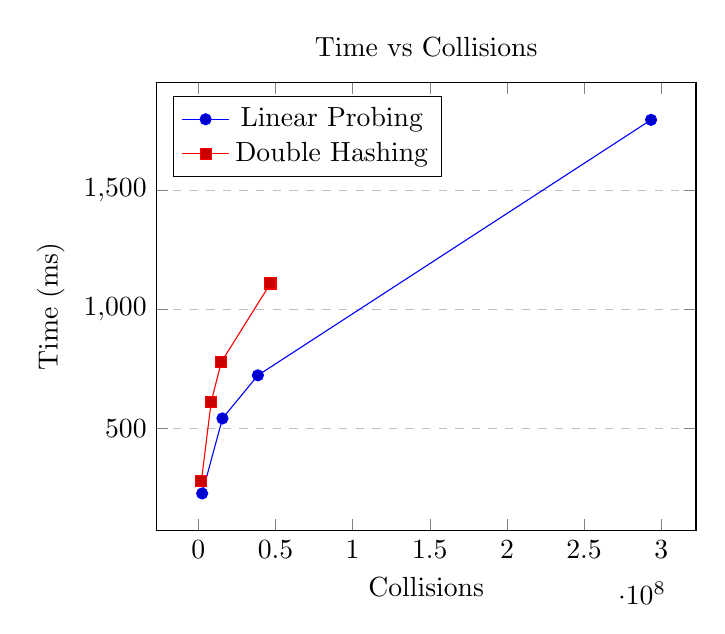
\begin{tikzpicture}
        \begin{axis}[
            title={Time vs Collisions},
            xlabel={Collisions},
            ylabel={Time (ms)},
            legend pos=north west,
            ymajorgrids=true,
            grid style=dashed,
        ]
        
        \addplot coordinates {
            (2450043, 227)
            (15601418, 542)
            (38560263, 723)
            (293414184, 1796)
        };
        \addlegendentry{Linear Probing}
        
        \addplot coordinates {
            (1925374, 278)
            (8286508, 611)
            (14800364, 778)
            (46712940, 1109)
        };
        \addlegendentry{Double Hashing}
        
        \end{axis}
    \end{tikzpicture}
    \caption{Forholdet mellom tid og antall kollisjoner ser ut til å være logaritmisk.}
\end{figure}


\section{Konklusjon}
Det tar betydelig mer tid for høyere fyllingsgrad og antall kollisjoner ser ut til å ha et omtrent logaritmisk forhold til tid. Dobbel hash er betydelig raskere enn lineær probing.

\end{document}
